\section{Ricerca della costante elastica della molla: metodo dinamico}

\subsection{Apparato sperimentale}

L'apparato sperimentale e la strumentazione utilizzata per compiere questo secondo esperimento, è la stessa utilizzata per la procedura del metodo statico, eccezion fatta per il cronometro. Il cronometro da noi utilizzato è un normale cronometro con risoluzione di misura di 0.01 s.

\subsection{Studio qualitativo e analisi dimensionale}

Come prima cosa abbiamo verificato in maniera qualitativa le relazioni che intercorrono tra
costante elastica della molla, massa applicata, ampiezza dell'oscillazione e periodo di oscillazione. I risultati sono stati
i seguenti:

\begin{itemize}
    \item{A parità di altre condizioni, all'aumentare della massa il periodo dell'oscillatore aumenta.}
    \item{A parità di altre condizioni, le molle più ''morbide`` (con costante elastica più bassa), hanno periodi più lunghi
        di molle più rigide (con costante elastica maggiore).}
    \item{A parità di altre condizioni, l'ampiezza dell'oscillazione non fa variare il periodo della molla. Questo significa
        che il periodo non dipende dall'ampiezza dell'oscillazione.}
\end{itemize}

\paragraph{Analisi dimensionale\\}

Con un analisi dimensionale è possibile ricavare una formula che metta in relazione periodo, massa e costante elastica della molla.
Per quanto visto sopra, supponiamo che il periodo $\mathcal{T}$ dipenda dalla massa $m$ appesa alla molla, dalla costante elastica $k$
e dall'ampiezza $A$ dell'oscillazione. Si ha quindi che $\mathcal{T} \propto m^\alpha k^\beta A^\gamma$. Facendo un analisi dimensionale:

\begin{equation*}
    [\mathcal{T}]^1 \,=\, [M]^{\alpha+\beta} [L]^\gamma [T]^{-2\beta} \quad \implies \quad \gamma = 0; \,\, \beta = -1/2; \,\, \alpha = 1/2
\end{equation*}
%
da cui si segue che

\begin{equation}
	\mathcal{T} \,=\, \mathcal{C} \, \sqrt{\frac{m}{k}}
    \label{eq:pp}
\end{equation}
%
dove $\mathcal{C}$ rappresenta una costante che non può essere determinata mediante l'analisi dimensionale. Come ci si poteva aspettare
dall'analisi qualitativa il periodo non dipende dall'ampiezza dell'oscillazione.

\subsection{Procedura di acquisizione dei dati}

Per calcolare la costante elastica mediante il metodo dinamico ci siamo avvalsi della relazione (\ref{eq:pp})
ricavata dall'analisi dimensionale.

Per le misurazioni sono state usate le stesse masse e le stesse combinazioni di cilindri scelte nell'esperimento precedente, con una sola differenza: è stata aggiunta una nuova configurazione di pesi di massa complessiva 135 g. Il numero totale delle configurazioni è quindi salito a 14.
Nella formula (\ref{eq:pp}), $m$ indica la massa complessiva che viene agganciata alla molla, quindi in questo caso si è dovuto tener conto della massa del piattello portapesi. Per evitare di dover propagare gli errori, abbiamo quindi misurato nuovamente la massa delle combinazioni
con l'aggiunta del piattello. Le masse nominali e pesate sono riportate nella tabella \ref{tab:masse_dinamico}.

Abbiamo quindi appeso le masse scelte alla molla e la abbiamo fatta oscillare.
Per ottenere il periodo di oscillazione abbiamo agito come segue:

\begin{itemize}
	\item{Si è deciso di cronometrare dieci oscillazioni della molla
        poichè abbiamo ritenuto di non essere in grado di rilevare con una precisione
        accettabile il periodo di una singola oscillazione. Questo metodo ha inoltre
        il pregio di un fattor dieci la risoluzione dello strumento.}

	\item{Per ogni massa sono state rilevate 15 misure di periodo.
        Ogni componente del gruppo ha cronometrato cinque cicli di dieci oscillazioni. 
        In questo modo gli errori sistematici dovuti alla prontezza di riflessi degli
        operatori dovrebbero essere misurabili o quantomeno visibili.}
\end{itemize}

I valori di lettura del cronometro sono stati divisi per dieci per ottenere i valori reali di periodo dell'oscillatore.
I dati rilevati sono riportati nella tabella \ref{tab:periodi}.

\begin{table}
    \centering
    \scriptsize
    \begin{tabular}{l | c c c c c c c c c c c c c c}
        \multicolumn{15}{c}{\small \textbf{Masse delle combinazioni di cilindri [g]}} \\[1mm]
        \toprule
        Nominali & 30 & 40 & 50 & 60 & 70 & 80& 90 & 100 & 110 & 120 & 130 & 140 & 150 & 160 \\
        Pesate & 30.3 & 40.3 & 50.2 & 60.3 & 70.4 & 80.3 & 90.5 & 100.3 & 110.4 & 120.4 & 130.4 & 140.4 & 150.5 & 160.5 \\
        \bottomrule
    \end{tabular}
    \caption{La tabella riporta le masse nominali e le masse rilavate con la bilancia delle combinazioni di pesi scelte per
    l'esperimento. Le masse includono il piattello portapesi e i cilindri delle combinazioni.}
    \label{tab:masse_dinamico}
\end{table}

\begin{table}
    \centering
    \scriptsize
    \begin{tabular}{l | c c c c c c c c c c c c c c c}
        \multicolumn{16}{c}{\small \textbf{Periodi}} \\[1mm]
        \toprule
        {\footnotesize Massa [g]} & \multicolumn{15}{c}{\footnotesize Periodi di oscillazione della molla [s]} \\
        \midrule
		30.3 & 3.84 & 3.90 & 3.95 & 3.95 & 3.99 & 3.91 & 3.91 & 3.93 & 3.90 & 3.94 & 4.04 & 3.92 & 4.00 & 3.98 & 3.95 \\
		40.3 & 4.38 & 4.43 & 4.43 & 4.45 & 4.41 & 4.54 & 4.45 & 4.49 & 4.50 & 4.56 & 4.49 & 4.52 & 4.47 & 4.49 & 4.41 \\
		50.2 & 4.84 & 4.76 & 4.85 & 4.92 & 4.87 & 4.93 & 4.88 & 4.78 & 4.83 & 4.82 & 4.95 & 5.02 & 4.93 & 4.99 & 4.78 \\
		60.3 & 5.29 & 5.33 & 5.27 & 5.24 & 5.30 & 5.27 & 5.30 & 5.21 & 5.25 & 5.27 & 5.30 & 5.34 & 5.34 & 5.31 & 5.34 \\
		70.4 & 5.65 & 5.65 & 5.64 & 5.63 & 5.59 & 5.63 & 5.64 & 5.63 & 5.66 & 5.63 & 5.81 & 5.67 & 5.63 & 5.63 & 5.65 \\
		80.3 & 5.98 & 5.98 & 5.95 & 5.98 & 5.95 & 6.01 & 6.08 & 6.02 & 5.98 & 5.95 & 5.98 & 5.99 & 6.06 & 6.09 & 6.07 \\
		90.5 & 6.33 & 6.34 & 6.32 & 6.34 & 6.32 & 6.33 & 6.26 & 6.31 & 6.31 & 6.31 & 6.34 & 6.35 & 6.37 & 6.34 & 6.34 \\
		100.3 & 6.58 & 6.63 & 6.56 & 6.59 & 6.56 & 6.63 & 6.69 & 6.64 & 6.58 & 6.63 & 6.63 & 6.68 & 6.63 & 6.57 & 6.69 \\
		110.4 & 6.86 & 6.96 & 6.93 & 6.94 & 6.84 & 6.91 & 6.86 & 6.99 & 6.96 & 6.94 & 6.99 & 6.84 & 6.94 & 6.95 & 6.88 \\
		120.4 & 7.24 & 7.20 & 7.22 & 7.23 & 7.20 & 7.18 & 7.23 & 7.13 & 7.24 & 7.23 & 7.24 & 7.21 & 7.27 & 7.26 & 7.24 \\
		130.4 & 7.53 & 7.51 & 7.45 & 7.52 & 7.56 & 7.53 & 7.52 & 7.57 & 7.52 & 7.52 & 7.56 & 7.55 & 7.53 & 7.46 & 7.50 \\
		140.4 & 7.81 & 7.78 & 7.76 & 7.74 & 7.74 & 7.73 & 7.79 & 7.82 & 7.81 & 7.74 & 7.79 & 7.79 & 7.73 & 7.78 & 7.79 \\
		150.5 & 8.02 & 7.94 & 8.04 & 8.06 & 8.07 & 8.12 & 8.02 & 8.05 & 7.98 & 8.04 & 7.99 & 7.93 & 8.02 & 7.99 & 8.02 \\
		160.5 & 8.30 & 8.27 & 8.15 & 8.29 & 8.25 & 8.24 & 8.35 & 8.31 & 8.41 & 8.27 & 8.36 & 8.34 & 8.34 & 8.31 & 8.31 \\
        \bottomrule
    \end{tabular}
    \caption{Periodi di oscillazione misurati con masse diverse. Ogni riga riporta le 15 misure effettuate per la massa
    riportata nella prima colonna della riga stessa. Sono riportati i valori di lettura del cronometro, relativi a 10
    periodi.}
    \label{tab:periodi}
\end{table}

\subsection{Elaborazione dei dati}

\subsubsection{Studio quantitativo del moto oscillatorio}

Nel grafico in figura \ref{fig:periodo_massa} sono riportati i risultati delle misure

Come si può notare dalla formula (\ref{eq:pp}) il periodo di oscillazione della molla è proporzionale alla radice di $m$. Se la costante elatica $k$ della molla è una costante e la legge è corretta, allora ci si dovrebbe aspettare che il periodo cresca al crescere della massa appesa, ma non con una proporzionalità diretta poichè la massa risulta essere sotto radice.]

\begin{SCfigure}
    \centering
    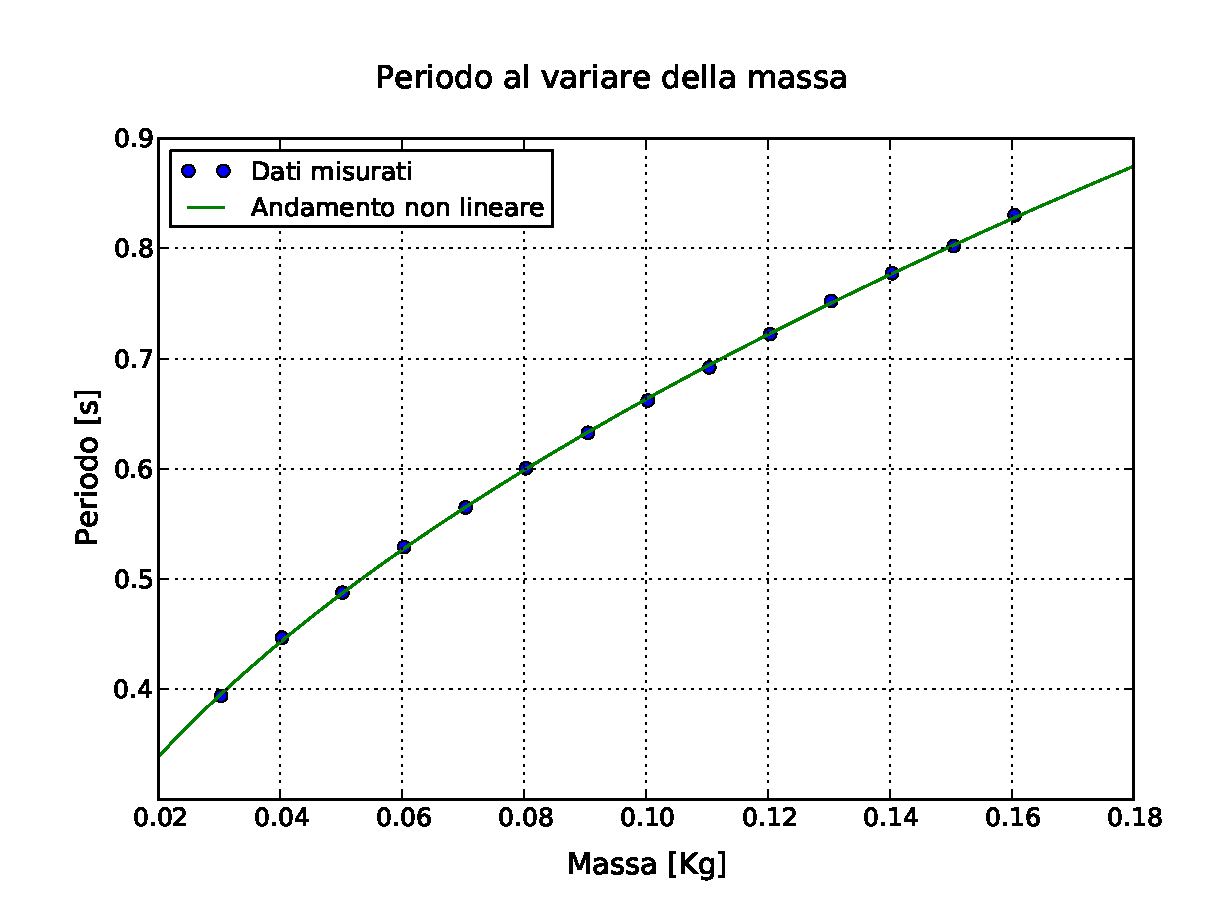
\includegraphics[width=120mm]{immagini/periodo_massa.pdf}
    \caption{Grafico}
    \label{fig:periodo_massa}
\end{SCfigure}

[principalmente servono grafici e tabelle. la parte di commento è molto ridotta]
\subsubsection{Massa efficace della molla}
Grazie ai grafici del paragrafo precedente possiamo notare che la retta che meglio interpreta i punti sperimentali nel grafico che rappresenta $\mathcal{T}^2$ in funzione della massa non passa per l'origine, ma interseca l'asse delle ascisse in corrispondenza di un valore negativo che definiamo come $- m_e$, che è la massa efficace della molla.
Noi sappiamo che un molla in sospensione a riposo è comunque soggetta a uno sforzo in quanto, avendo un propria massa, le spire sono sottoposte alla forza peso dovuta alla molla stessa. Questo effetto apparentemente complicato si può semplificare affermando che lo sforzo compiuto dalla molla può essere paragonato all'effetto che darebbe una massa di valore ($m_e$) appesa alla molla. Pertanto grazie allo studio del grafico abbiamo trovato un valore della massa efficace che risulta essere:

\begin{equation*}
	m_e \,\,=\,\, 8 grammi
\end{equation*}
%
Per questo motivo è doveroso modificare l'equazione

\begin{equation*}
	\mathcal{T} \,=\, \mathcal{C} \, \sqrt{\frac{m}{k}}
\end{equation*}
%
sostituendo a m (la massa allpicata) con $M = m + m_e$ per cui noi otteniamo quanto segue:

\begin{equation*}
	\mathcal{T} \,=\, \mathcal{C} \, \sqrt{\frac{M}{k}}
\end{equation*}
%
e quindi la legge lineare che dipende da $\mathcal{T}^2$ e dalla massa (M) data dalla somma dei carichi applicati (m) e la massa efficace della molla ($m_e$).

\subsubsection{Calcolo dei parametri $\mathcal{C}$ e $m_e$ mediante il metodo della regressione lineare}
Prendiamo in considerazione la seguente legge:

\begin{equation*}
	\mathcal{T}^2 \,\,=\,\, \frac{\mathcal{C}^2}{k} m_e \,+\, \frac{\mathcal{C}^2}{k} m
\end{equation*}
%
la cui scrittura può essere semplificata nel seguente modo:

\begin{equation*}
	y \,=\, A \,+\, Bx
\end{equation*}
%
dove $x \equiv m$ (massa appesa) $y \equiv \mathcal{T}^2$, $A \equiv \frac{\mathcal{C}^2}{k} m_e$ e $B \equiv \frac{\mathcal{C}^2}{k}$.
Vogliamo quindi determinare i valori di A e B che minimizzano la discrepanza mediante la tecnica della regressione lineare pertanto procediamo con il metodo utilizzato anche nella sezione due.
\begin{itemize}
\item{calcoliamo la discrepanza:
		\begin{equation*}
			discrepanza \,=\, \sum_{i=1}^{13} \frac{(y_i - A - Bx_i)^2}{(\delta y_i)^2}
		\end{equation*}
		%
		ricordando che l'incertezza sull'asse delle ascisse è la stessa incertezza sulla massa ovvero $\delta m_i$ che in questa analisi poniamo uguli a $\delta x_i$ e che risulta trascurabile [è vero?????] rispetto all'incertezza che dellasse delle ordinate $\delta y_i \equiv \delta \mathcal{T}^2$}
\item{quindi per quanto studiato in classe abbiamo che:
		\begin{equation*}
			A \,=\, \frac{(\sum_i w_i x_i^2)(\sum_i w-i y_i) - (\sum_i w_i x_i)(\sum_i w_i x_i y_i)}{\Delta} \,=\,
		\end{equation*}
		%
		\begin{equation*}
			B \,=\, \frac{(\sum_i w_i)(\sum_i w-i x_i y_i) - (\sum_i w_i y_i)(\sum_i w_i x_i)}{\Delta} \,=\,
		\end{equation*}
		%
		dove:
		\begin{equation*}
			\Delta \,=\, (\sum_i w_i)(\sum_i w_i x_i^2) - (\sum_i w_i x_i)^2 \,\,\,\,\,\,\, e \,\,\,\,\,\,\,
			w_i \,=\, \frac{1}{(\delta y_i)^2}
		\end{equation*}}
\item{di conseguenza abbiamo che le incertezze relative su A e B sono:

		\begin{equation*}
			(\delta A)^2 \,=\, \frac{\sum_i w_i x_i^2}{\Delta} \,=\,  \,\,\,\,\, e \,\,\,\,\,
			(\delta B)^2 \,=\, \frac{\sum_i w_i}{\Delta} \,=\,
		\end{equation*}}
\end{itemize} 
Quindi possiamo riassumere i risultati di questa procedura in questo modo:

\begin{equation*}
	A \,\pm\, \delta A \,=\, \pm \,\,\,\,\, e \,\,\,\,\,
	B \,\pm\, \delta B \,=\, \pm
\end{equation*}
Perciò noti questi parametri possiamo risalire ai valoti di $\mathcal{C}$ e $k$ risolvendo l'equazione in (... inizio ...) e utilizzando come valore di k quello trovato nell'analisi dati della sezine precedente ovvero $K = ...$

\subsubsection{Test del chi quadro}
Procediamo ora a verificare che i valori sopra ottenuti siano compatibili con i dati sperimentali mediante il test del chi quaro. Ricordiamo che il numero di gradi di libertà in questo caso non è più N - 1, ma risulta essere N - 2 in qunto due dati sono stati utilizzati per calcolare i datisperimentali A e B. Pertanti ci aspettiamo che:

\begin{equation*}
	\chi^2 \,=\, \sum_{i=1}^{N} \frac{(y_i - A - Bx_i)^2}{(\delta y_i)^2} \,\simeq\, N - 2
\end{equation*}
%





